\documentclass[10pt]{beamer}

\usepackage[utf8]{inputenc}
\usepackage[T1]{fontenc}
\usepackage[french]{babel}
\usepackage[ddmmyyyy]{datetime}
\usepackage{listings,lstautogobble,graphicx,tikz}
\usepackage{lmodern}
\usetikzlibrary{arrows,automata}
\usetikzlibrary{positioning}

\usetheme{Warsaw}
\useinnertheme{rectangles}
\setbeamerfont{headline}{size=\large}
\setbeamerfont{frametitle}{size=\normalsize}

%Plan/Sommaire automatique avant chaque section
\AtBeginSection[]{
  \begin{frame}
  \frametitle{Plan}
  \tableofcontents[currentsection]
  \end{frame}
}

\author{Jean-Didier Pailleux - Robin Feron - Romain Robert - Damien Thenot - Maxence Joulin}
\institute{UVSQ}
\date{\today}
\usepackage{../tex/myInfolines}
\usepackage{longtable,array}
\title{Test de Primalité}

\begin{document}
	\begin{frame}
		\titlepage
	\end{frame}
	
	\section*{Introduction}
        \begin{frame}
            \begin{itemize}
            \item \textbf{Nombre Premier:} Entier divisible par 1 et lui-même.\\pause
            \vspace{1em}            
            \item \textbf{Test Probabiliste:}Test avec marge d'erreur très faible mais rapide.  \\
            \vspace{1em}
            \item \textbf{ Test Deterministe:} Test fiable mais plus lent.    \\
            \vspace{1em}
            \item \textbf{$2^{64}$:}Taille maximale des nombre a tester => Unsigned long long int  \\
            \vspace{1em}
            \item \textbf{Nombre Hautement Composé:}Entier qui possède strictement plus de diviseur que les nombres qui le précède\\
            \end{itemize}            
        \end{frame}
	
	\begin{frame}
		\tableofcontents
	\end{frame}
	
	\section{Architecture}
		\begin{frame}
	Qui ?
		\end{frame}
		
	\section{{\small Outils et Langage de Programmation}}
		\begin{frame}
	Qui ?
		\end{frame}
		
	\section{Analyse des Résultats}
		\begin{frame}
		\textbf{Fonctionnement du projet :}

	\begin{itemize}
		\item Script appelé avec ./test.sh\\
\textbf{Options :}


	\begin{center}\footnotesize\begin{longtable}{l l}		
	\textbf{a} : Tous les algorithmes  & \textbf{k} : AKS\\
	\textbf{e} : Euclide (computation bound) & \textbf{o} : Modulo (computation bound)\\
	\textbf{m} : Crible d'eratosthene & \textbf{p} : Pocklington\\
	\textbf{i} : Miller-Rabin & \textbf{h} : Nombre hautement composé naive\\
	\textbf{H} : Nombre hautement composé def\\
	\end{longtable}\vspace{-2.2em}\end{center}

		\item Lequel utiliser ?\\
		\item Itération ?\\
		\item Combien de nombre ?\\
		\item Donner les nombres\\
	\end{itemize}
		\end{frame}
		\begin{frame}
		\textbf{Evolution du temps d'exécution de Eratosthène/Memory Bound: }
		\begin{center}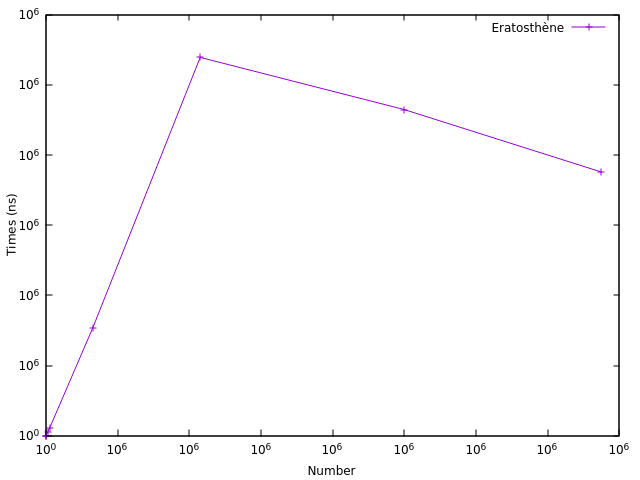
\includegraphics[scale=0.6]{eratosthene.png}\end{center}
		\end{frame}
		
		\begin{frame}
		\textbf{Evolution du temps d'exécution de Euclide/Computation Bound: }
		\begin{center}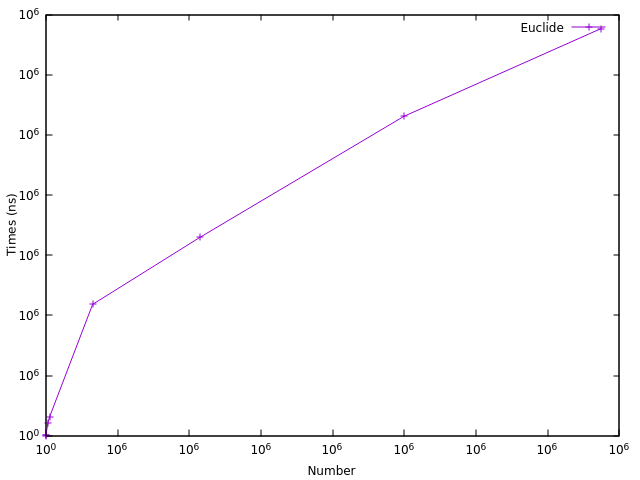
\includegraphics[scale=0.6]{euclide.png}\end{center}
		\end{frame}
		
		\begin{frame}
		\textbf{Evolution du temps d'exécution de Modulo/Computation Bound: }
		\begin{center}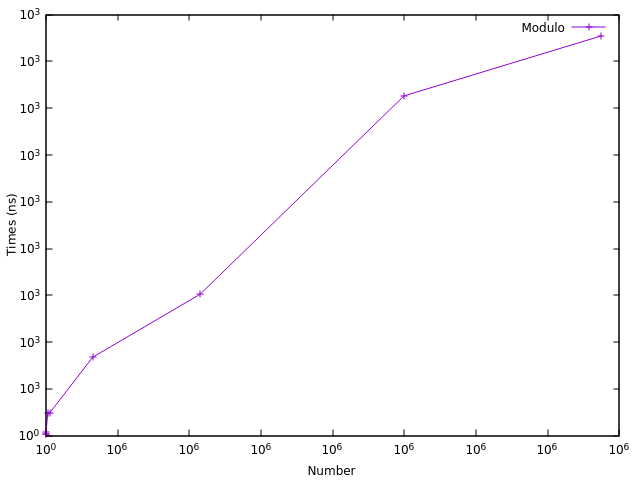
\includegraphics[scale=0.6]{modulo.png}\end{center}
		\end{frame}
		
		\begin{frame}
		\textbf{Evolution du temps d'exécution d'AKS: }
		\begin{center}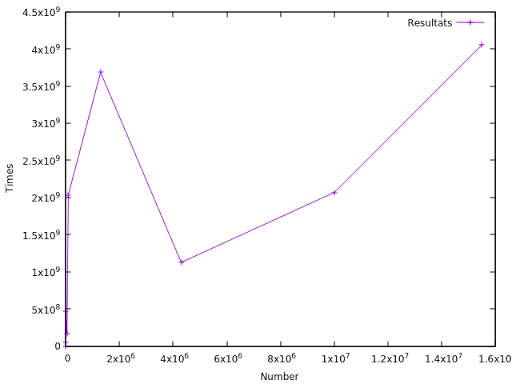
\includegraphics[scale=0.6]{AKS.png}\end{center}
		\end{frame}
		
		\begin{frame}
		\textbf{Evolution du temps d'exécution de Pocklington: }
		\begin{center}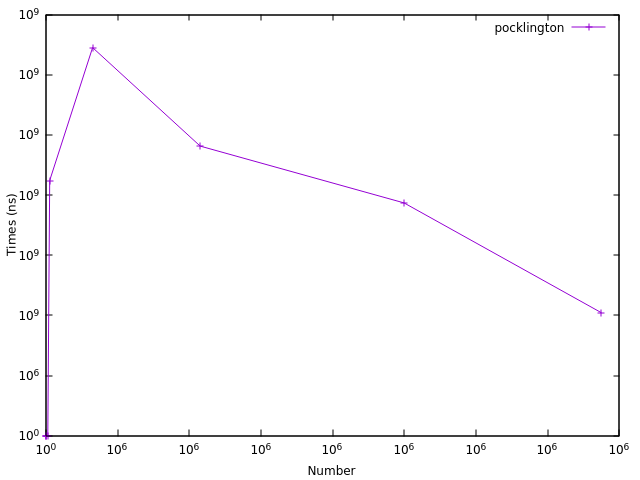
\includegraphics[scale=0.6]{pocklington.png}\end{center}
		\end{frame}
		
		\begin{frame}
		\textbf{Evolution du temps d'exécution de Miller-Rabin: }
		\begin{center}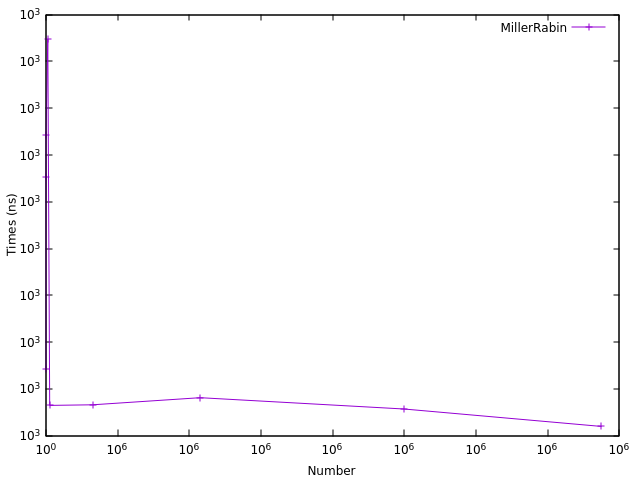
\includegraphics[scale=0.6]{miller.png}\end{center}
		\end{frame}
		
		\begin{frame}
		\textbf{Evolution du temps d'exécution de Hautement composé (méthode naïve et définition): }
		
		\footnotesize\begin{longtable}{l l}		
	\hspace{-2em}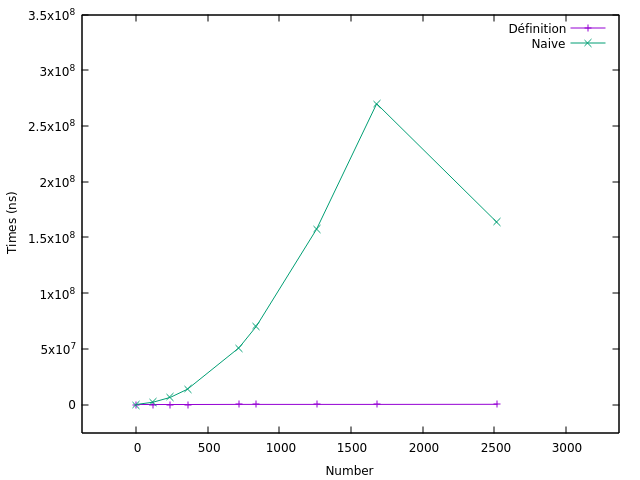
\includegraphics[scale=0.27]{HC.png}  & 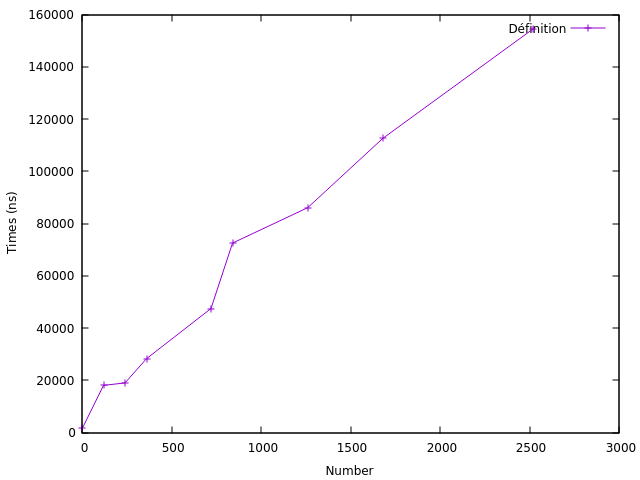
\includegraphics[scale=0.27]{HCdef.png}\\
	\end{longtable}
		\end{frame}
		
		\begin{frame}
		\begin{center}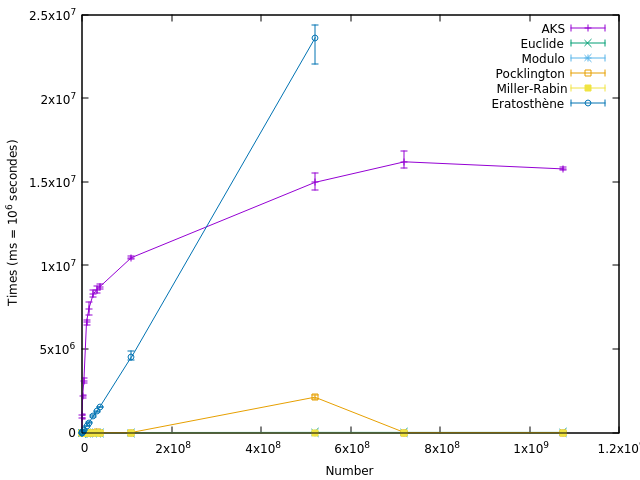
\includegraphics[scale=0.6]{result.png}\end{center}
		\end{frame}
		
	\section{Bilan Technique}
		\begin{frame}
			\begin{itemize}
			\item \textbf{crible d'Eratosthène/ Mémory Bound:} Création d'un tableau de taille N+1 dans le crible => limité au niveau de la RAM pour N grand sur nos machines. Complexité de N pour le remplissage de la liste memory\_bound. \\
			\vspace{1em}			
			\item \textbf{Computation Bound:} Effectue $\sqrt{2^{log_2(n)}}$ divisions euclidiennes => Exécution en temps exponentiel\\
			\vspace{1em}
			\item \textbf{Pocklington:} Limite causé par la factorisation du nombre N-1 => facotisation très longues pour N très grand.\\
			\vspace{1em}
			
			\end{itemize}	
			\end{frame}
			
			\begin{frame}
			\begin{itemize}
			\item \textbf{Miller-Rabin:} Résultats faux dans certains cas + Nombre d'itérations demandé élevé pour un meilleur résultat => augmentation du temps d'exécution.  \\
			\vspace{1em}
			\item \textbf{AKS:} \underline{Avantage:} Sa complexité en $log(n)^{12}$.\\
						\underline{Inconvénient:} Utilisation de NTL qui effectue des vérifications superflue + Implémentation compliquée.\\
			\vspace{1em}
			\item \textbf{Hautement Composé:} N calcul du nombre de diviseurs d'un nombre => exécution très lente pour la méthode naïve.\\
			\end{itemize}			
		\end{frame}
		
	\section{Organisation interne du groupe}
	\begin{frame}
\textbf{Tableau de répartition du travail:} \\
	
	\begin{center}\vspace{-1em}\footnotesize\begin{longtable}{|>{\centering}m{3.0cm}|>{\centering}m{1.5cm}|>{\centering}m{1.2cm}|>{\centering}m{1.2cm}|>{\centering}m{1.2cm}|>{\centering\arraybackslash}m{1.2cm}|}			
		\hline \multicolumn{1}{|c|}{\textbf{Tâches}} & \multicolumn{1}{c|}{\textbf{Jean-Didier}} & \multicolumn{1}{ c|}{\textbf{Maxence}} & \multicolumn{1}{ c|}{\textbf{Romain}} & \multicolumn{1}{ c|}{\textbf{Robin}} & \multicolumn{1}{c|}{\textbf{Damien}}\\
		\hline 	Eratosthène/Memory Bound & x & ~ & ~ & ~ & ~ \\
		\hline 	Euclide/Computation Bound & ~ & x & ~ & ~ & ~ \\
		\hline 	AKS & ~ & ~ & x & ~ & ~ \\
		\hline 	Pocklington & ~ & ~ & ~ & ~ & x \\
		\hline 	Miller-Rabin & ~ & ~ & ~ & x & ~ \\
		\hline 	Highly Composite & x & ~ & ~ & ~ & ~ \\
		\hline 	Cmake  & x & x & ~ & ~ & ~ \\
		\hline  Script & x & x & ~ & ~ & ~ \\
		\hline
	\end{longtable}\vspace{-2.2em}\end{center}
	\end{frame}
	\section{Conclusion}
		\begin{frame}
	 \begin{itemize}
        \item De gros temps de calculs \vspace{2em}
        \item Difficultés d'implémentations \vspace{2em}
        \item Possibilités de parallélisation \vspace{2em}
     \end{itemize}
		\end{frame}	
		
\end{document}
